\documentclass{report}
\usepackage{graphics}
\usepackage{subfig}
\usepackage[T1]{fontenc}
\usepackage[utf8]{inputenc}
\usepackage[french]{babel}
\usepackage{amsfonts,amssymb,amsmath,amsthm}
\usepackage{graphicx}

\begin{document}
On propose une autre association courbe discrete - courbe continue que celle proposée par Lachaud avec les normales.

Sur la frontière discrete, on distingue deux type de sommets (voir Fig.~\ref{sfig:tube1}):
\begin{itemize}
\item
  entre deux arêtes alignées ; le sommet est alors le centre d'un carré dont deux sommets adjacents sont allumés et les deux autres sont éteints.
\item
  entre deux arêtes orthogonales ; le sommet est alors le centre de l'hypothénuse d'un triangle rectangle isocèle dont l'angle droit est éteint et les deux autres sommets allumés, ou inversement.
\end{itemize}
  
\begin{figure}[!h]
  \centering
  \subfloat[]{\label{sfig:tube1}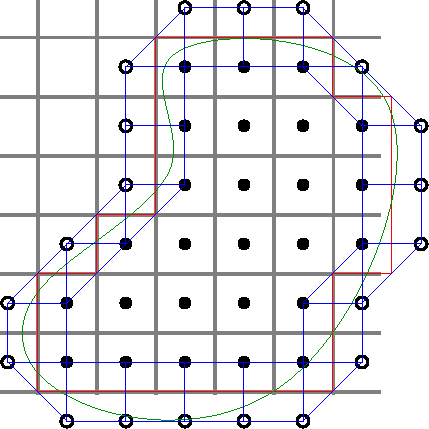
\includegraphics[scale=0.65]{tube.pdf}}
  \hspace{1cm}
  \subfloat[)]{\label{sfig:tube3}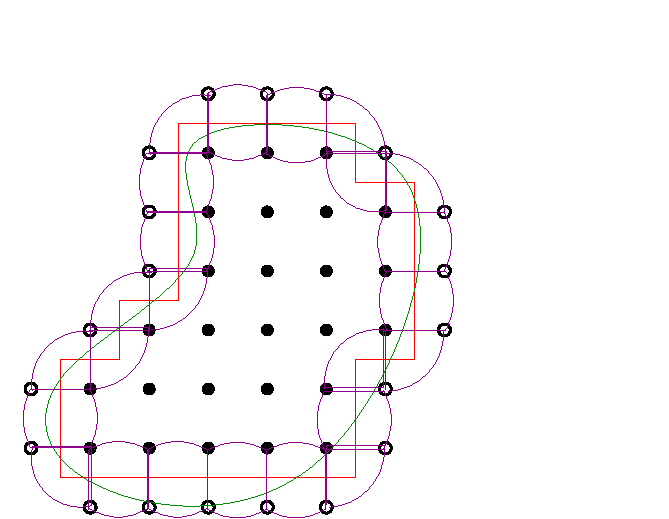
\includegraphics[scale=0.65,clip=true,trim=0 0 100 40]{tube3.pdf}}
  \caption{\label{fig:tube}(a) En vert : la courbe continue. Points noirs : discrétisation de Gauss (points allumés). Points blancs : points éteints. En rouge : la courbe discrète. En bleu : les carrés et triangles décrits dans le texte.
  (b) Idem avec des \og carrés\fg{} et des \og triangles\fg{} qui tiennent compte de la courbure maximale de la courbe.}
\end{figure}


En prenant comme hypothèse la par($r$)-regularité et $h<r$, on devrait pouvoir montrer que la courbe est tout entière incluse dans l'union de ces carrés et triangles sous reserve de les gonfler un peu comme sur la figure~\ref{fig:carres_triangles}. Le \og tube\fg{} obtenu est affiché sur la figure~\ref{sfig:tube3}.
\begin{figure}[h!]
  \centering
  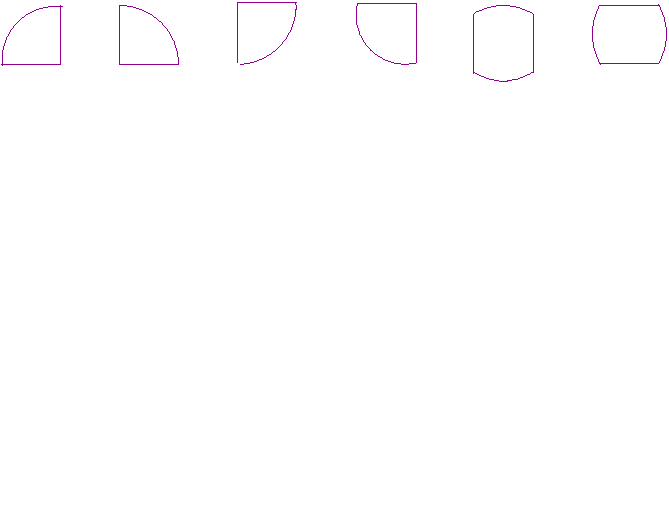
\includegraphics[width=8cm,clip=true,trim=0 210 0 0]{tube3-1}
    \caption{\label{fig:carres_triangles}Les arcs de cercle ont pour rayon $r$ avec ici $r=h$ soit le minimum puisque, par hypothèse, $h<r$.}
    \end{figure}

    Sous reserve d'arriver à montrer que l'intersection de la courbe avec une structure carré ou triangle est connexe, on associera à chaque sommet de la courbe discrète le centre (relativement à la paramétrisation) du segment de courbe délimité par la structure associée au sommet. Pour l'instant, on nomme $\Pi$ cette association.

    \bigskip
    
    \hfill TSVP $\to$

    \newpage. 
    \paragraph{Parcours d'une structure carré}
    On se propose de montrer que la courbe ne franchit qu'une seule fois la \og porte d'entrée\fg{} d'une structure carré avant de ressortir de l'autre côté.
    Les notations sont celles de la figure~\ref{fig:normale_horiz}.

    \begin{proof}
      Soient $A$, $B$, $C$, $D$, les sommets de la structure carré. Raisonnons par l'absurde. Si la courbe franchit $[AD]$ une première fois puis une seconde fois avant d'avoir franchit la \og porte de sortie\fg{} $[BC]$, par le théorème des valeurs intermédiaires sur la composante horizontale de la dérivée, il existe un point dans la structure carré où la normale est horizontale (parallèle à $[AB]$).
      Soit $E$ un tel point. Les centres des boules tangentes intérieures et extérieures sont alors les points $F$ et $G$. Disons par exemple que $F$ est le centre de la boule tangente intérieure et $G$ le centre de la boule tangente extérieure. Alors, $F$ ne doit pas être dans le disque $d_D$ de centre $D$ et de rayon $h$ sinon la boule tangente intérieure contiendrait le point extérieur $D$. De même, $G$ ne doit pas être dans le disque $d_B$ de centre $B$ et de rayon $h$.
      On en déduit que $E$ ne peut pas être dans le translaté de $d_D$ de vecteur $\vec {FE}$, c'est-à-dire dans le disque $d_C$ de centre $C$ et de rayon 1 ni, symétriquement, dans le disque $d_A$ de centre $A$ et de rayon 1. Comme l'union de ces deux derniers disques recouvrent la structure carré, le point $E$ appartient à l'ensemble vide.
    \end{proof}
    
    \begin{figure}[!h]
      \centering
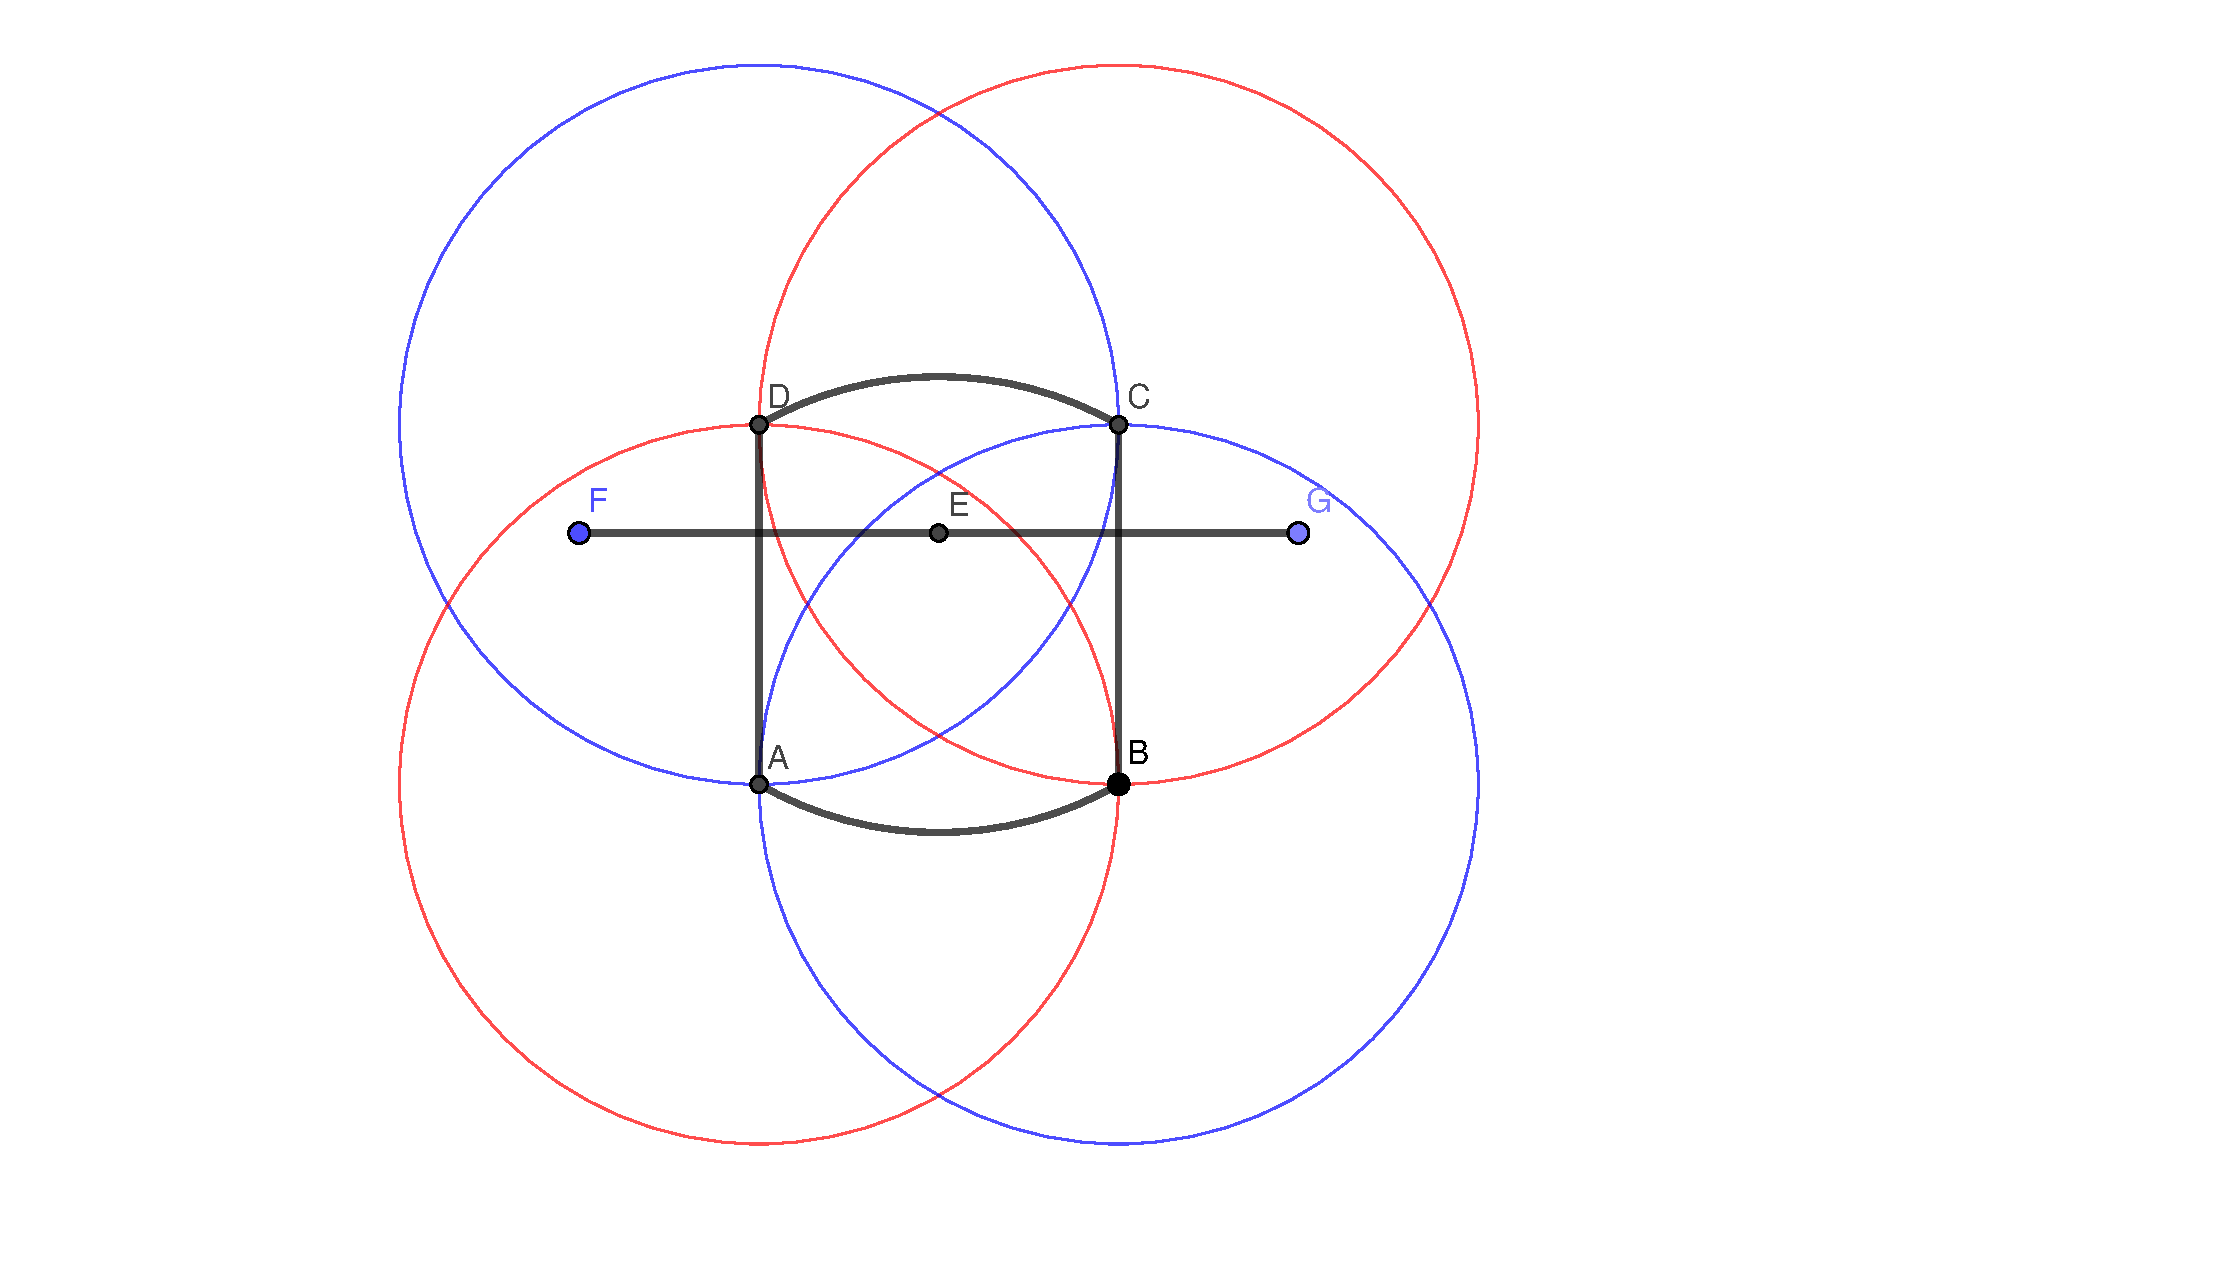
\includegraphics[width=12cm]{normale_horiz.pdf}
\caption{\label{fig:normale_horiz}Tous les cercles ont pour rayon $h$ et les segments $[AB]$, $[BC]$, $[CD]$, $DA]$, $[EF]$ et $[EG]$ ont pour longueur $h$.}
\end{figure}

La propriété précédente devrait permettre de montrer une propriété de croissance de l'association sommet discret $\to$ point sur courbe : si les sommets discrets $x$, $y$, $z$ sont tels que $y$ est entre $x$ et $z$ alors $\Pi(y)$ est entre $\Pi(x)$ et $\Pi(z)$.

\end{document}
